\section{Introduction}
The challanges at hadron collider experiments are many, one of the
most well known is the fact the the energy and momentum of the parton-parton
(hard) interaction is not know. This limitation, in addition with the
fact that a large number of the proposed extensions of the SM (e.g. SUSY) predict
new particles that are weakly interacting and therefore escape the
detector systems without a trace, have made events with large momentum
imbalance in the plane transverse to the beam a key signature to
search for BSM physics. The momentum imbalance is the transverse plane
(missing energy)
is quantified by $\ptvecmiss$  which is defined as 
\begin{equation}
\label{eq:ptmiss}
\ptvecmiss = -\sum\limits_{i=0}^{n_{pf}} \vec{p}_{T}^{\hspace{0.06cm}i},
\end{equation}
where $\vec{p}_{T}^{\hspace{0.06cm}i}$ is the measured transeverse
momentum of a PF candidate, and $n_{pf}$ is the total number of PF
candidates reconstructed.

Additionally, in SUSY models with R-parity conservation the originally
pair produced super-partners undergo a cascade decay and at least two
particles (the LSPs) will escape detection and therefore further reduce the
hability to fully reconstruct the event kinematics due to the lost
information. Subsequently, all these effects result in lost of
sensitivity as the discrimination power between a possible
signal and the SM background processes is reduced. In order to recover
sensitivity, different kinematic variables are employed which are
functions of the visible objects momenta and the $\ptvecmiss$. These
kinematic variables have been shown to improve signal to background
discrimination but are often model dependent. One example of such
variables arew the razor variables~\cite{rogan,razor2010}, which have been widely used by the
CMS collaboration to search for
SUSY~\cite{Chatrchyan:2014goa,Razor8TeV} and recently shown to have
good sensitivity for DM direct production at hadron
colliders~\cite{Fox:2012ee}. The razor variables: $\MR$ and $\RR^2$  provide an estimate of the
underlying mass scale of the event and a handle to significantly
supress SM backgrounds -- particularly QCD multiijet --,
respectively. 

Since the two searches for BSM physics presented in this thesis are
based on the razor variables, this Chapter describes its derivation
(see Section~\ref{razorVariables})
and their main features when searching for new physics (see Section~\ref{razorApp}).

\section{The Razor Variables}\label{razorVariables}
The razor variables were originally derived~\cite{rogan,razor2010} for
squark pair-production in the context of SUSY; this topology is
represented by the Feynman diagram shown in Figure~\ref{fig:squarkpair}, where
the proton-proton collision pair produces two squarks ($\tilde{q}_{1}\tilde{q}_{2}$) which
subsequently decay into a SM quark and the LSP ($\tilde{q}_{i}\rightarrow q_{i}\tilde{\chi}_{1}^{0}$).

\begin{figure}
 \centering
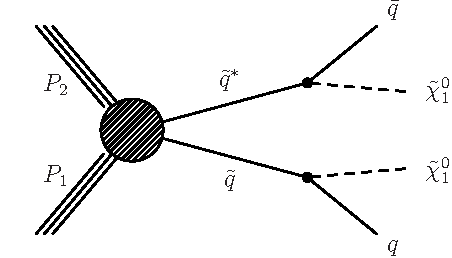
\includegraphics[width=0.4\textwidth]{RazorVariables/T2qq.pdf}
 \caption{Feynman diagram for squark pair-production.\label{fig:squarkpair}}
\end{figure}
One interesting quantity that provides access to the mass scale of the
SUSY particles is the magnitude of the 3-momentum of the quark in the
rest frame of the squark, it is actually more convenient to write down
twice this quantity:
\begin{equation}
\label{eq:pq}
2|\vec{p}^{\hspace{0.06cm}q_{i}}| =
2|\vec{p}^{\hspace{0.06cm}\tilde{\chi}_{1}^{0}}| =
\frac{\sqrt{m^{4}_{\tilde{q}} -
2m^{2}_{\tilde{q}}m^{2}_{\tilde{\chi}_{1}^{0}} +
m^{4}_{\tilde{\chi}_{1}^{0}} - 2m^{2}_{q}m^{2}_{\tilde{\chi}_{1}^{0}}
- 2m^{2}_{q}m^{2}_{\tilde{q}} + m_{q}^{4}}}{m_{\tilde{q}}},
\end{equation}
 where $m_{\tilde{q}}$ is the squark mass, $m_{\tilde{\chi}_{1}^{0}}$
 is the LSP mass, and $m_{q}$ is the SM quark mass. Eq.~\ref{eq:pq}
 can be simplified if the SM quarks are assumed massless -- which is
 mostly accurate with the exception of the top-quark. This
 simplification is also useful to define:
\begin{equation}
\label{eq:Mdelta}
M_{\Delta} = 2|\vec{p}^{\hspace{0.06cm}q_{i}}| =
\frac{m^{2}_{\tilde{q}} -
m^{2}_{\tilde{\chi}_{1}^{0}}}{m_{\tilde{q}}}.
\end{equation}

$M_{\Delta}$ is sensitive to the mass-splitting between the squark and
the LSP  and therefore is usually refer to as the characteristic mass
scale of the event. For example, in the case of the $W\rightarrow
\ell\nu$ decay, $M_{\Delta}$ is simply the mass of the W boson.

The razor variable \MR provides an estimate of $M_{\Delta}$ by
approximating the boosts needed -- since the actual boosts are
imposible to reconstruct due to the missing particles, which can be
viewed as an undetermined system of equations with not enough
contraints -- to go from the laboratory frame (lab frame) to the
squark rest frame. This approximation is done in two steps, first
, there is a common boost to go from the lab frame to the
center-of-momentum (CM) frame, and then, an equal and opossite boost
applied to each squark to go from the CM frame to their respective
rest frame. Figure~\ref{fig:restFrames} depicts the three frames and
the boosts needed to move from the lab frame to the squark rest frames.
\begin{figure}
 \centering
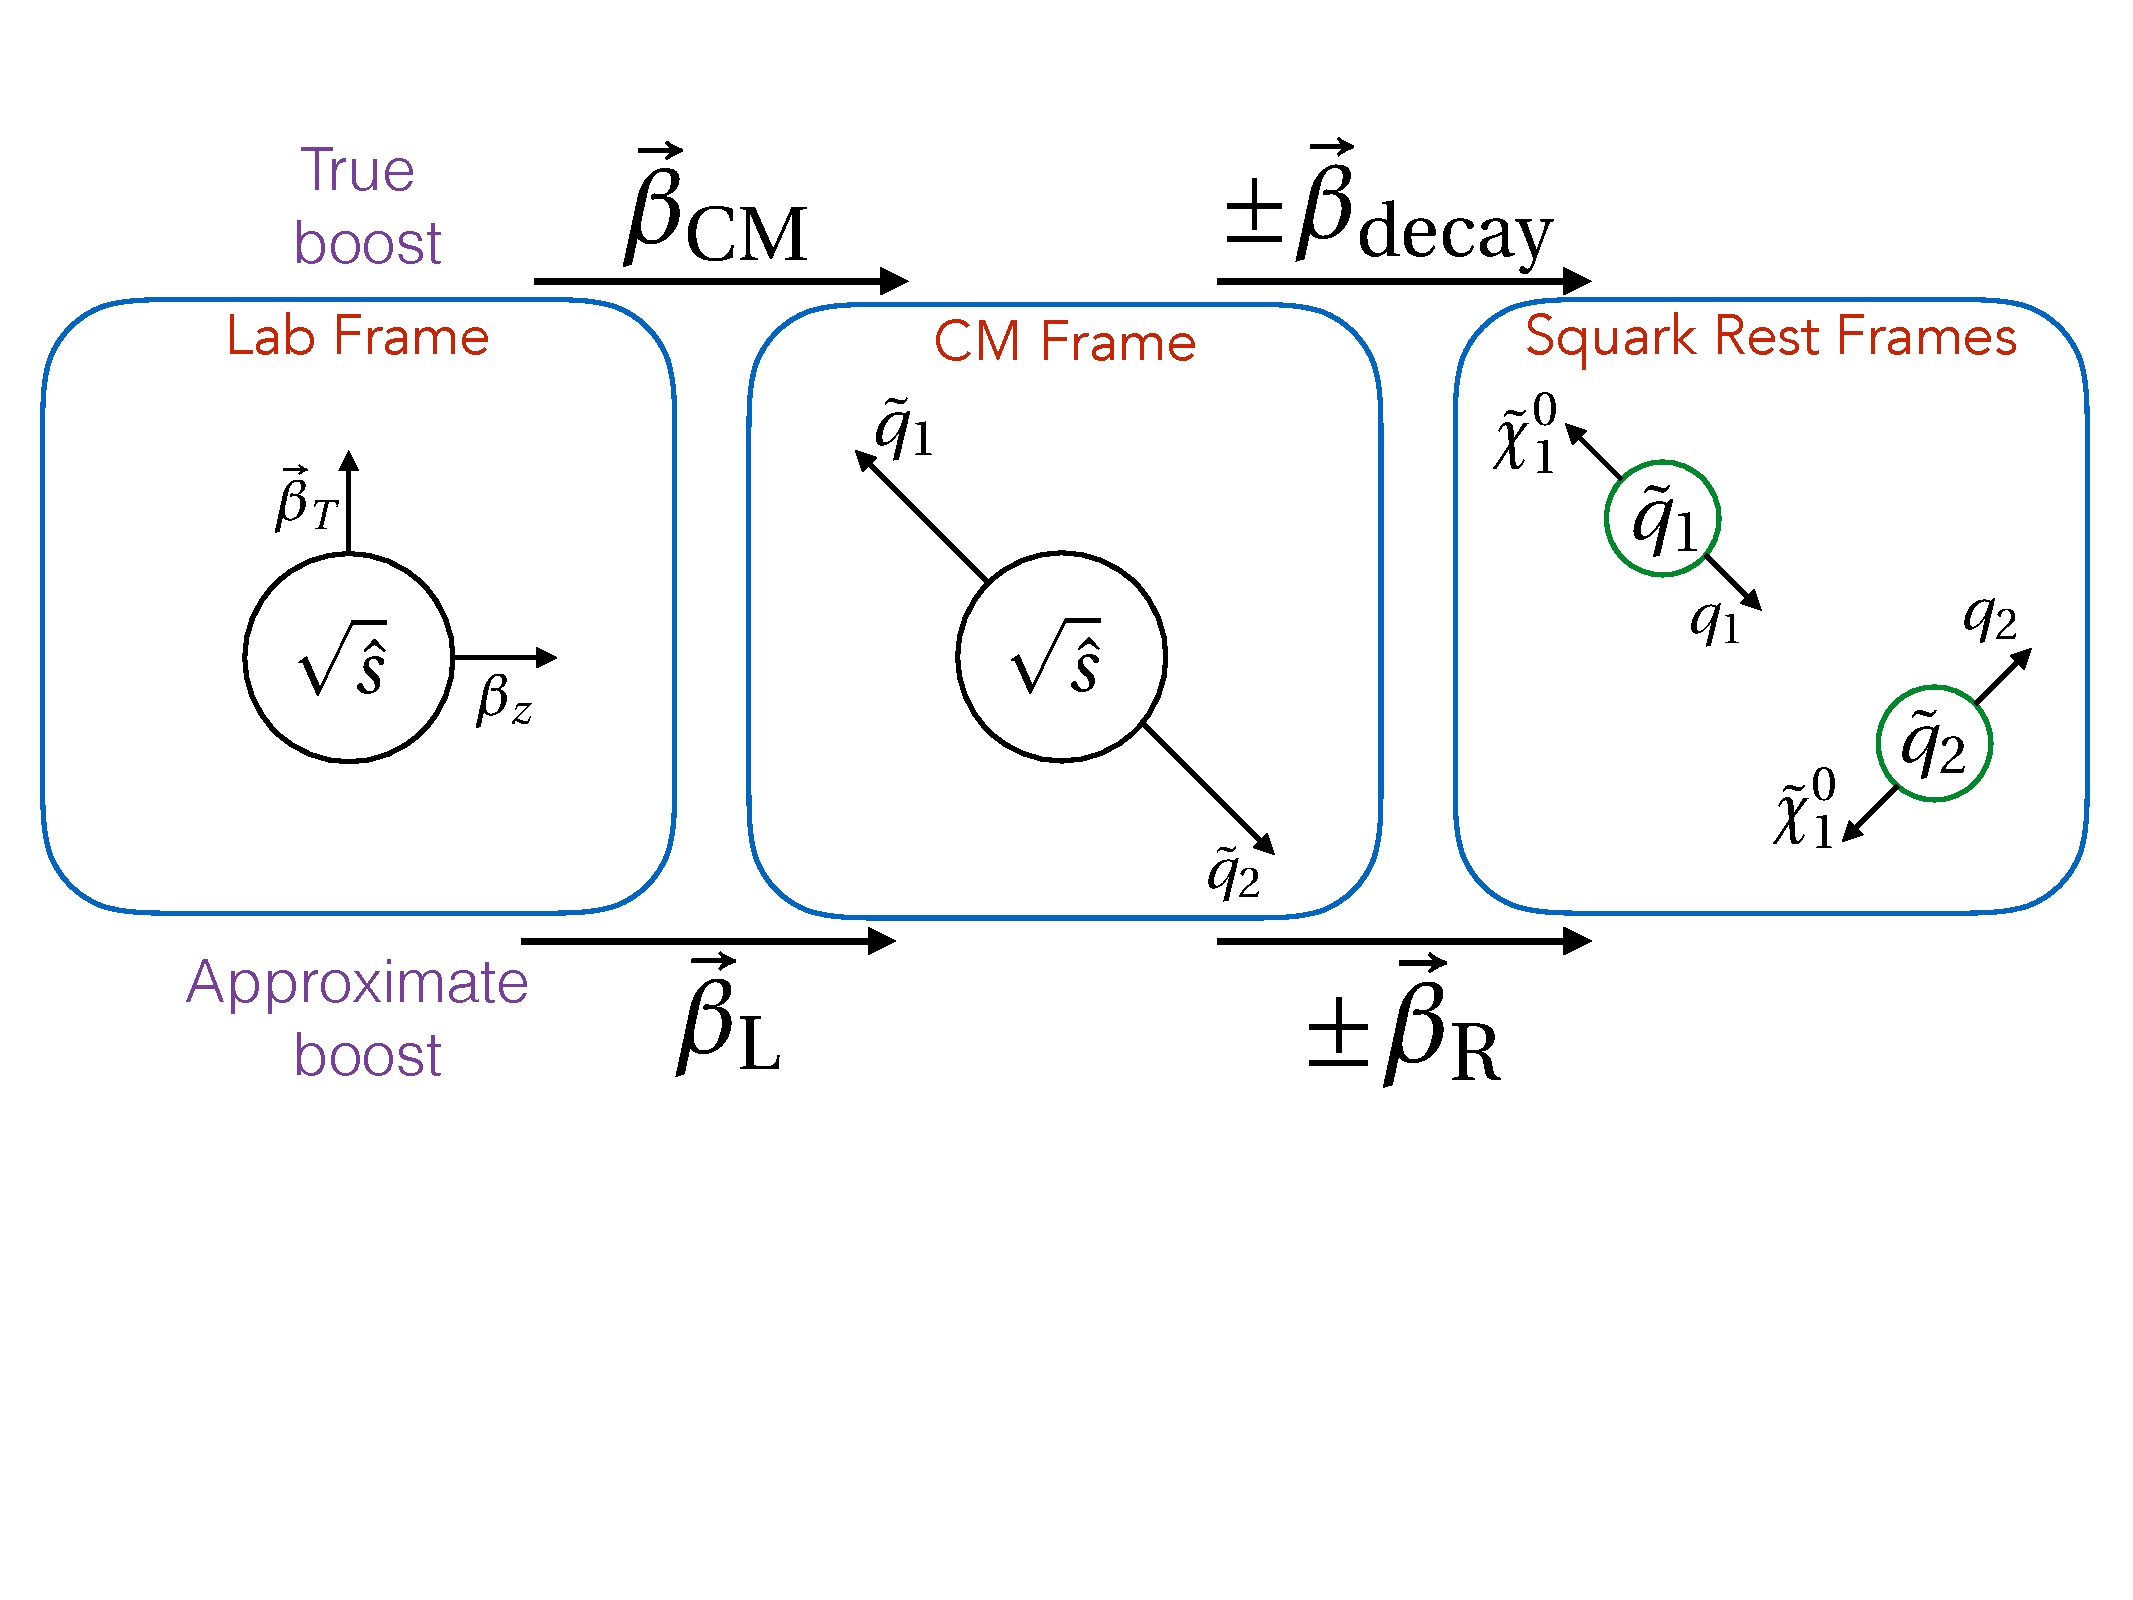
\includegraphics[width=1.0\textwidth]{RazorVariables/RazorFrameDiagram.pdf}
 \caption{An schematic of the  different rest frames involved in
   deriving the razor variables. The lab frame is in the left panel,
   the CM frame is in the middle panel, and the  squark rest frames
   are in the right panel.\label{fig:restFrames}}
\end{figure}  


\section{Application of the Razor Variables to Search for BSM Physics}\label{razorApp}

